\chapter{Apartado C: \textbf{Filtro de Kalman para Seguimiento de Objetos}}
\label{chapter:tarea_c}

\section*{Tarea C.1: Configuración del Filtro de Kalman}
\phantomsection
\addcontentsline{toc}{section}{Tarea C.1: Configuración del Filtro de Kalman}
Para esta tarea vamos a utilizar el video \texttt{'slow\_traffic\_small.mp4'}. Para cargarlo utilice el método que se ha desarrollado anteriormente. Inicialice el filtro de Kalman, para ello haga uso del método \texttt{cv2.KalmanFilter}\footnote{ \href{https://docs.opencv.org/4.8.0/dd/d6a/classcv_1_1KalmanFilter.html}{Documentación del método KalmalFilter en OpenCV:} \\{https://docs.opencv.org/4.8.0/dd/d6a/classcv\_1\_1KalmanFilter.html}} de Opencv, con una matriz de medición y transición adecuada para un seguimiento en dos dimensiones.

Complete el código del bucle que nos permitirá seleccionar el objeto \texttt{(cv2.selectROI)}\footnote{ \href{https://docs.opencv.org/4.8.0/d7/dfc/group\_\_highgui.html\#gaabb58bae304674b429d9102a7155a86e}{Documentación del método para seleccionar la ROI en OpenCV:} \\{https://docs.opencv.org/4.8.0/d7/dfc/group\_\_highgui.html\#gaabb58bae304674b429d9102a7155a86e}} que vamos a seguir. Convierta la región de interés de la imagen a HSV y calcule el histograma \texttt{cv2.calcHist}\footnote{ \href{https://docs.opencv.org/4.8.0/d6/dc7/group\_\_imgproc\_\_hist.html\#ga4b2b5fd75503ff9e6844cc4dcdaed35d}{Documentación del método para calculo de histograma en OpenCV:} \\{https://docs.opencv.org/4.8.0/d6/dc7/group\_\_imgproc\_\_hist.html\#ga4b2b5fd75503ff9e6844cc4dcdaed35d}} con  para el canal con la información de tono (\textit{Hue}).

\begin{figure}[H]
    \centering
    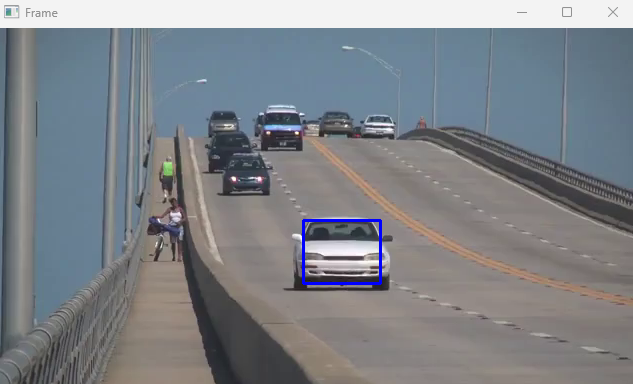
\includegraphics[width=0.45\textwidth]{Lab_4/template/figures/roi_selection.png}
    \caption{Ejemplo de ROI.}
    \label{fig:ejemplo_ROI_kalman}
\end{figure}

\section*{Tarea C.2: Predicción y Corrección del Estado}
\phantomsection
\addcontentsline{toc}{section}{Tarea C.2: Predicción y Corrección del Estado}
Realice la predicción del estado y corrija la posición estimada en cada iteración.

\begin{figure}[H]
    \centering
    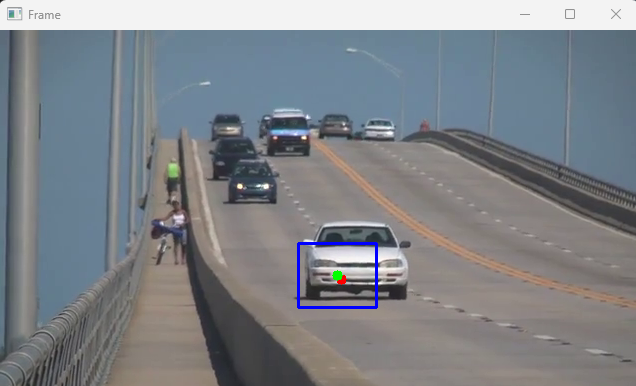
\includegraphics[width=0.45\textwidth]{Lab_4/template/figures/kalman.png}
    \caption{Ejemplo de seguimiento con filtro de Kalman.}
    \label{fig:ejemplo_track_kalman}
\end{figure}

\section*{Preguntas}
\addcontentsline{toc}{section}{Preguntas}

\vspace{5mm}
\begin{tcolorbox}[colback=gray!10, colframe=gray!30, coltitle=black, title=Pregunta C.1, halign=left]
¿Cómo afecta el valor de \texttt{transitionMatrix} a la predicción en el filtro de Kalman?
\end{tcolorbox}

\vspace{5mm}
\begin{tcolorbox}[colback=gray!10, colframe=gray!30, coltitle=black, title=Pregunta C.2, halign=left]
¿Cuál es la diferencia entre \texttt{measurementMatrix} y \texttt{transitionMatrix} en el contexto del seguimiento de objetos?
\end{tcolorbox}